\begin{topic}{polyhedral-cone}{polyhedral cone}
    A \textbf{polyhedral cone} in $\RR^n$ is a set of the form
    \[ \sigma = \{ \lambda_1 v_1 + \cdots + \lambda_r v_r : \lambda_i \in \RR_{\ge 0} \} , \]
    for some $v_1, \ldots, v_r \in \RR^n$. The vectors $v_1, \ldots, v_r$ are called \textit{generators} of the polyhedral cone $\sigma$.
    
    The polyhedral cone $\sigma$ is called \textbf{rational} if the generators $v_i$ can be chosen to lie in $\ZZ^n$.
    
    The polyhedral cone $\sigma$ is called \textbf{strongly convex} if $\sigma \cap (-\sigma) = \{ 0 \}$.
    
    The \textit{dimension} of $\sigma$ is the dimension of the linear subspace spanned by $\sigma$.
    
    A \textit{face} of $\sigma$ is an intersection $\tau = \sigma \cap u^\perp = \{ v \in \sigma \;|\; \langle u, v \rangle = 0 \}$ for some $u \in \sigma^\vee$, where $\sigma^\vee$ denotes the \tref{dual-cone}{dual cone} of $\sigma$.
\end{topic}

\begin{example}{polyhedral-cone}
    Consider the following polyhedral cones in $\RR^2$.
    \[ 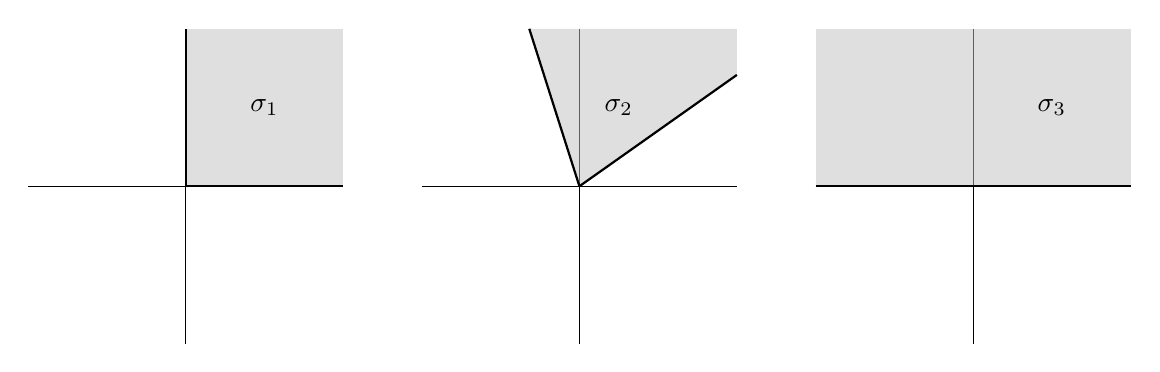
\begin{tikzpicture}
        \begin{scope}[shift={(-5,0)}]
            \draw (-2, 0) -- (2, 0);
            \draw (0, -2) -- (0, 2);
            \fill[fill=gray!50, opacity=0.5] (0, 0) -- (0, 2) -- (2, 2) -- (2, 0);
            \draw[thick] (0, 0) -- (2, 0);
            \draw[thick] (0, 0) -- (0, 2);
            \node at (1, 1) {$\sigma_1$};
        \end{scope}
        \begin{scope}
            \draw (-2, 0) -- (2, 0);
            \draw (0, -2) -- (0, 2);
            \fill[fill=gray!50, opacity=0.5] (0, 0) -- (2, 1.4142135) -- (2, 2) -- (-0.63661977, 2);
            \draw[thick] (0, 0) -- (2, 1.4142135);
            \draw[thick] (0, 0) -- (-0.63661977, 2);
            \node at (0.5, 1) {$\sigma_2$};
        \end{scope}
        \begin{scope}[shift={(5,0)}]
            \draw (-2, 0) -- (2, 0);
            \draw (0, -2) -- (0, 2);
            \fill[fill=gray!50, opacity=0.5] (-2, 0) -- (2, 0) -- (2, 2) -- (-2, 2);
            \draw[thick] (0, 0) -- (2, 0);
            \draw[thick] (0, 0) -- (-2, 0);
            \node at (1, 1) {$\sigma_3$};
        \end{scope}
    \end{tikzpicture} \]
    The above cones are given by
    \[ \sigma_1 = \RR_{\ge 0} \{ (1, 0), (0, 1) \}, \quad \sigma_2 = \RR_{\ge 0} \{ (\sqrt{2}, 1), (-1, \pi) \}, \quad \sigma_3 = \RR_{\ge 0} \{ (-1, 0), (1, 0) \} .  \]
    Cones $\sigma_1$ and $\sigma_3$ are rational, while $\sigma_2$ is not. Cones $\sigma_1$ and $\sigma_2$ are strongly convex, while $\sigma_3$ is not. All cones have dimension $2$. The faces of $\sigma_1$ are $\{ \{ 0 \}, \RR_{\ge 0} (1, 0), \RR_{\ge 0} (0, 1), \sigma_1 \}$.
\end{example}

\begin{topic}{dual-cone}{dual cone}
    The \textbf{dual cone} of a \tref{polyhedral-cone}{rational polyhedral cone} $\sigma \subset \RR^n$ is
    \[ \sigma^\vee = \{ u \in (\RR^n)^* : \langle u, v \rangle \ge 0 \text{ for all } v \in \sigma \} . \]
\end{topic}

\begin{example}{dual-cone}
    For any polyhedral cone $\sigma \subset \RR^n$, we have $(\sigma^\vee)^\vee = \sigma$. Indeed, it is clear from the definition that $\sigma \subset (\sigma^\vee)^\vee$. Conversely, if $v \not\in \sigma$, then there exists some $u \in \sigma^\vee$ with $\langle u, v \rangle < 0$, so that $v \not\in (\sigma^\vee)^\vee$.
\end{example}

\begin{topic}{fan}{fan}
    A \textbf{fan} in $\RR^n$ is a set $\Delta$ of \tref{polyhedral-cone}{rational strongly convex polyhedral cones}, such that
    \begin{itemize}
        \item every face of a cone in $\Delta$ is also a cone in $\Delta$,
        \item the intersection of two cones in $\Delta$ is a face of each.
    \end{itemize}
\end{topic}

\begin{topic}{gordons-lemma}{Gordon's lemma}
    Let $M$ be a \tref{GT:finitely-generated-group}{finitely generated} \tref{GT:free-group}{free abelian group}, and $\sigma \subset M_\RR = M \otimes_\ZZ \RR$ a \tref{polyhedral-cone}{rational polyhedral cone}. Then \textbf{Gordon's lemma} states that the \tref{AA:monoid}{commutative monoid} $M \cap \sigma$ is finitely generated.
\end{topic}

\begin{example}{gordons-lemma}
    \begin{proof}
        Write $\sigma = \left\{ \sum_{i = 1}^{s} \lambda_i v_i : \lambda_i \in \RR_{\ge 0} \right\}$ for some $v_i \in M$, and let
        \[ K = \left\{ \sum_{i = 1}^{s} t_i v_i : 0 \le t_i \le 1 \right\} \subset M_\RR . \]
        Then $K$ is compact, and since $M$ is discrete, $K \cap M$ is finite. Now take any $u \in M \cap \sigma$, and write $u = \sum_{i = 1}^{s} r_i v_i$ for some $r_i \in \RR_{\ge 0}$. Write $r_i = n_i + t_i$ with $n_i \in \NN$ and $t_i \in [0, 1)$. Then,
        \[ u = \sum_{i = 1}^{s} n_i v_i + \sum_{i = 1}^{s} t_i v_i . \]
        Hence, $M \cap \sigma$ is generated by the $v_i$ and all $K \cap M$.
    \end{proof}
\end{example}

\begin{example}{gordons-lemma}
    Consider $M = \ZZ^2$ and $\sigma = \RR_{\ge 0} \langle (1, 2), (2, 1) \rangle \subset \RR^2$. Gordon's lemma tells us that $M \cap \sigma$ is finitely generated, in particular by the elements $K \cap M = \{ (0, 0), (1, 1), (1, 2), (2, 1), (2, 2), (3, 3) \}$. We can further reduce this to a generating set $\{ (1, 1), (1, 2), (2, 1) \}$.
\end{example}
